% $Id$
%

\section{La API de los servicios de Google}

%%---------------------------------------------------------------

\begin{frame}
\frametitle{La(s) API(s) de los servicios de Google}

\begin{itemize}
  \item Google ofrece una API para acceder a muchos servicios
  \item Algunas APIs son de pago
  \item Otras tienen limitaciones de uso gratuito
  \item Hay peticiones que requieren autenticación y autorización
\end{itemize}

\end{frame}

%%---------------------------------------------------------------

\begin{frame}
\frametitle{El API Explorer (I)}

Google ofrece un servicio para explorar sus APIs, el API Explorer:

\begin{itemize}
  \item Permite conocer los métodos de las APIs
  \item Permite probarlos mediante un formulario web
  \item A veces requieren autorización/autenticación
  \item Incluyen un enlace a la documentación completa
\end{itemize}

APIs Explorer: https://developers.google.com/apis-explorer/\#p/

\end{frame}


%%---------------------------------------------------------------

\begin{frame}
\frametitle{El API Explorer (II)}

\begin{center}
\begin{figure}[p]
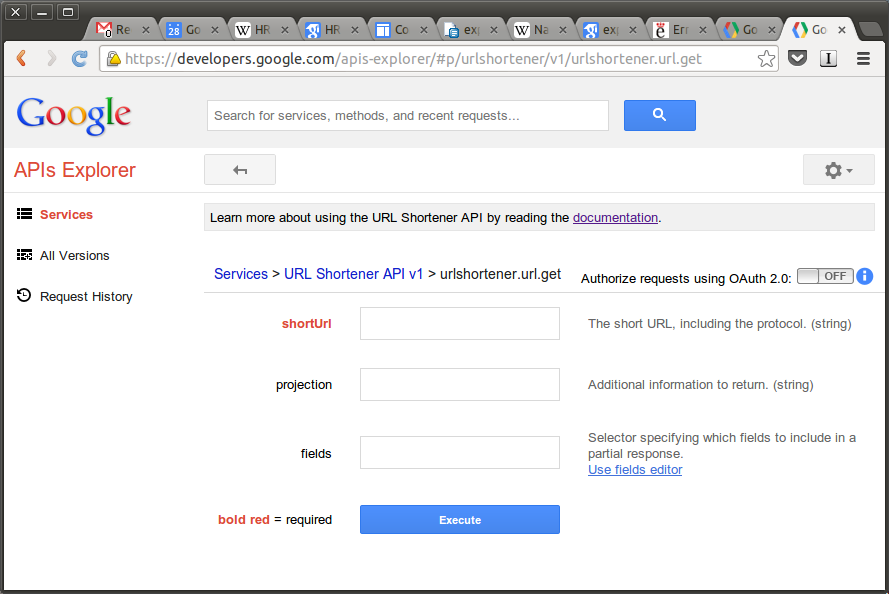
\includegraphics[width=0.8\textwidth]{figs/apiexplorer.png}
\end{figure}
\end{center}

\end{frame}

%%---------------------------------------------------------------

\begin{frame}
\frametitle{Ejemplo de uso del API Explorer}

Utilicemos el API Explorer para el servicio de acortadores de URLs de Google.

\begin{itemize}
  \item En el campo \emph{shortUrl}, introduce \emph{http://goo.gl/JCHYE}
  \item Pulsa el botón Execute
  \item Observa la petición: es una petición HTTP REST
  \item Observa la respuesta: es en formato JSON
\end{itemize}

\end{frame}

%%---------------------------------------------------------------

\begin{frame}
\frametitle{La Google API Console}

Es una interfaz web para gestionar el uso de la API de Google en tu proyecto.
Permite:

\begin{itemize}
  \item Activar APIs
  \item Obtener la llave (\emph{project key}) que se envía al utilizar la API, gestionar autenticación y autorización
  \item Obtener información de tráfico (y ver las cuotas de uso)
  \item Gestionar cobros
  \item Gestionar miembros del equipo
\end{itemize}

\end{frame}


%%---------------------------------------------------------------

\begin{frame}
\frametitle{Ejercicio: Google API Console}

Crea un proyecto para utilizar la Google API Console.

\begin{itemize}
  \item Selecciona los servicios de Google+ API y URL Shortener API
  \item Obtén tu \emph{project key}
  \item Añade como \emph{referer} http://watson.gsyc.es/
  \item Incluye información de autorización vía OAuth2.0, también para http://watson.gsyc.es/
  \item Échale un ojo a los menús de \emph{Reports} y \emph{Quotas}
\end{itemize}

Nota: Para realizar este ejercicio (y los siguientes), necesitarás tener
una cuenta en Google.

\end{frame}

\section{La API de Google+}

%%---------------------------------------------------------------

\begin{frame}[fragile]
\frametitle{La API de Google+}

\begin{itemize}
  \item Google+ ofrece una API REST para acceder a los contenidos de la red social
  \item Hay varios lenguajes soportados, entre ellos Javascript
  \item Los navegadores modernos lo soportan:
  \begin{itemize}
    \item Chrome 8+
    \item Firefox 3.5+
    \item MSIE 8+
    \item Safari 4+
  \end{itemize}
\end{itemize}


\end{frame}

%%---------------------------------------------------------------

\begin{frame}
\frametitle{Referencia de la API de Google+}

Hay cuatro tipo de recursos, que vienen representados con una estructura
de datos JSON:

\begin{itemize}
  \item People
  \item Activities
  \item Comments
  \item Moments
\end{itemize}

Más información: https://developers.google.com/+/api/latest/

\end{frame}


%%---------------------------------------------------------------

\begin{frame}
\frametitle{Recursos}

Cada recurso cuenta con una serie de métodos. Por ejempo, el recurso
People tiene:

\begin{itemize}
  \item get
  \item search
  \item listByActivity
  \item list
\end{itemize}

Más información: https://developers.google.com/+/api/latest/people\#resource

\end{frame}


%%---------------------------------------------------------------

\begin{frame}
\frametitle{Estructura de un script Javascript}

\begin{enumerate}
  \item Se carga la biblioteca JavaScript
  \item Se indican los credenciales de acceso
  \item Se carga la API del servicio con el que queremos trabajar
  \item Se inicializa un objeto que encampsula la petición
  \item Se ejecuta el objeto petición
  \item Se procesa el resultado
\end{enumerate}

\end{frame}

%%---------------------------------------------------------------

\begin{frame}[fragile]
\frametitle{1. Cargando la biblioteca JavaScript}


\begin{footnotesize}
\begin{verbatim}
<script 
  src="https://apis.google.com/js/client.js?onload=OnLoadCallback">
</script>
\end{verbatim}
\end{footnotesize}

\begin{enumerate}
  \item Al producirse el evento, llama a la función \emph{callback} que se indica
\end{enumerate}


\end{frame}

%%---------------------------------------------------------------

\begin{frame}
\frametitle{2. Indicando credenciales (I)}

Hay dos tipos de acceso:

\begin{enumerate}
  \item Simple:
  \begin{itemize}
    \item Llamadas que no acceden a datos privados
    \item Hace falta enviar la \emph{API key}
  \end{itemize}
  \item Autorizada:
  \begin{itemize}
    \item Llamadas que leen o escriben datos privados o de la propia aplicación
    \item Hace falta un credencial OAuth 2.0
  \end{itemize}
\end{enumerate}

\end{frame}


%%---------------------------------------------------------------

\begin{frame}[fragile]
\frametitle{2. Indicando credenciales (I)}

Ejemplo de acceso simple:

\begin{footnotesize}
\begin{verbatim}
var apiKey = 'AIzaSyDy.......VbeXghdvuHDI8A'; // From API Console
gapi.client.setApiKey(apiKey);
\end{verbatim}
\end{footnotesize}

Ejemplo de acceso autorizado:

\begin{footnotesize}
\begin{verbatim}
// From the API Console
var clientId = '4764....7773'; 
// Services to be used
var scopes = 'https://www.googleapis.com/auth/plus.me'; 

gapi.auth.authorize({client_id: clientId, scope: scopes, immediate: true},
   callback_function);
\end{verbatim}
\end{footnotesize}

\texttt{callback\_function} es la función que se ejecutará una vez se haya obtenido
la autorización.

\end{frame}

%%---------------------------------------------------------------

\begin{frame}[fragile]
\frametitle{3. Cargar API del servicio}

\begin{verbatim}
gapi.client.load(API_NAME, API_VERSION, CALLBACK);
\end{verbatim}

donde:

\begin{itemize}
  \item API\_NAME es el nombre de la API
  \item API\_VERSION es la versión de la API
  \item CALLBACK es una función opcional a ejecutar cuando se haya cargado
\end{itemize}

Para cargar la versión 1 de la API de Google+:

\begin{verbatim}
gapi.client.load('plus', 'v1', function() {
   console.log('loaded.'); 
});
\end{verbatim}

\end{frame}


%%---------------------------------------------------------------

\begin{frame}[fragile]
\frametitle{4. Objeto que encampsula petición}

\begin{verbatim}
var ApiRequest = gapi.client.METHOD_NAME(PARAMETERS_OBJECT);
\end{verbatim}

donde:

\begin{itemize}
  \item METHOD\_NAME es un método de la API del servicio
  \item PARAMETERS\_OBJECT es un objeto con parámetros que dependerán 
del método utilizado
\end{itemize}

Por ejemplo, la siguiente llamada busca actividades cuyo título sea Google+:

\begin{verbatim}
var request = gapi.client.plus.activities.search(
  {'query': 'Google+', 'orderBy': 'best'}
);
\end{verbatim}


\end{frame}


%%---------------------------------------------------------------

\begin{frame}[fragile]
\frametitle{5. Ejecución del objeto petición}

\begin{verbatim}
ApiRequest.execute(callback);
\end{verbatim}

donde:

\begin{itemize}
  \item ApiRequest es un objeto que encapsula la petición (ver paso 4.)
  \item callback es la función que tratará la respuesta 
\end{itemize}

Por ejemplo:

\begin{verbatim}
request.execute(function(resp) { console.log(resp); });
\end{verbatim}

\end{frame}


%%---------------------------------------------------------------

\begin{frame}
\frametitle{6. Procesar el resultado}

\begin{itemize}
  \item La API devuelve dos objetos a la función callback:
  \begin{enumerate}
    \item jsonResp: un objeto JSON
    \item rawResp: un string con la respuesta HTTP
  \end{enumerate}
\end{itemize}

Cuando la respuesta no pueda ofrecerse como JSON, el valor de jsonResp será \emph{false}; pero rawResp seguirá ofreciendo la respuesta HTTP completa como string.


\end{frame}


